\documentclass{../../../oss-apphys-exam}
\newcounter{lastmc}

\begin{document}

\gentitle{11}{ROTATIONAL MOTION, PART 3}


\raggedcolumns

\runningheader{
  \fontfamily{phv}\small
  \textcolor{gray}{AP PHYSICS C: MECHANICS $\blacksquare$}
  \textbf{MULTIPLE-CHOICE QUESTIONS}}{}{}

\begin{questions}
    
  \question A hoop of radius $R$ and mass $m$ has a rotational inertia of
  $mR^2$. The hoop rolls without slipping along a horizontal floor with a
  constant speed $v$ and then rolls up a long incline. The hoop can roll up the
  incline to a maximum vertical height of
  \begin{center}
    \begin{tikzpicture}
      \fill[lightgray] (0,-.2) rectangle (7,0);
      \draw[thick] (0,0)--(7,0);
      \draw[thick] (3.5,0)--(7,1.2)--(7,0);
      \draw[thick] (1.5,.4) circle (.4);
      \fill (1.5,.4) circle (.06);
      \draw[vectors] (1.5,.4)--(2.5,.4) node[right]{$v$};
      \draw[vectors] (.95,.4) arc (180:45:.55);
      \draw[thick,|<->|] (7.2,0)--(7.2,1.2) node[midway,right]{$h$};
    \end{tikzpicture}
  \end{center}
  \begin{choices}
    \choice$\dfrac{v^2}g$
    \choice$\dfrac{2v^2}{g}$
    \choice$\dfrac{v^2}{2g}$
    \choice$\dfrac{4v^2}{g}$
    \choice$\dfrac{v^2}{4g}$
  \end{choices}
    
  \question A disk is mounted on a fixed axle. The rotational inertia of the
  disk is $I$. The angular velocity of the disk is decreased from $\omega_i$ to
  $\omega_f$ during a time $\Delta t$ due to friction in the axle. The
  magnitude of the average net torque acting on the wheel is
  \begin{choices}
    \choice $\dfrac{\omega_f-\omega_i}{\Delta t}$
    \choice $\dfrac{(\omega_f-\omega_i)^2}{\Delta t}$
    \choice $\dfrac{I(\omega_f-\omega_i)}{\Delta t}$
    \choice $\dfrac{I(\omega_f-\omega_i)^2}{\Delta t}$
    \choice $\dfrac{I(\omega_f-\omega_i)}{\Delta t^2}$
  \end{choices}
    
  \question The average power developed by the friction in the axle of the disk
  from the previous question to bring it to a complete stop is
  \begin{choices}
    \choice $\dfrac{\omega_i}{\Delta t}$
    \choice $\dfrac{\omega_i^2}{\Delta t}$
    \choice $\dfrac{I\omega_i}{2\Delta t}$
    \choice $\dfrac{I\omega_i^2}{2\Delta t}$
    \choice $\dfrac{I\omega_i}{\Delta t^2}$
  \end{choices}
  \newpage
  
  \question One end of a stick of length $L$, rotational inertia $I$, and mass
  $m$ is pivoted on an axle with negligible friction at point $P$. The other
  end is tied to a string and held in a horizontal position. When the string is
  cut, the stick rotates counterclockwise. The angular speed $\omega$ of the
  stick when it reaches the bottom of its swing is
  \cpic{.32}{end-of-stick}
  \begin{choices}
    \choice $\dfrac{mgL}I$
    \choice $\sqrt{\dfrac{mgL}I}$
    \choice $\sqrt{\dfrac{2mgL}I}$
    \choice $\sqrt{\dfrac{mgL}{2I}}$
    \choice $\sqrt{\dfrac{4mgL}I}$
  \end{choices}
  \newpage

  \runningheader{
    \fontfamily{phv}\small
    \textcolor{gray}{AP PHYSICS C: MECHANICS $\blacksquare$}
    \textbf{FREE-RESPONSE QUESTIONS}}{}{}


% TAKEN FROM THE 2015 AP PHYSICS C FREE-RESPONSE QUESTION MECH 3
%
%\begin{center}
%  \begin{tikzpicture}[scale=.8,thick]
%    \shade[ball color=lightgray] circle (2);% node[below right]{$m$};
%    \draw circle (2);
%    \fill circle (.15);
%    \draw (2,0)--(2,-4);
%    \draw[fill=gray!30] (1.5,-4) rectangle (2.5,-5) node[midway]{$m$};
%    \draw[vectors] (2,-4)--(2,-1.8) node[right]{$T$};
%  \end{tikzpicture}
%\end{center}

  \uplevel{
    \centering
    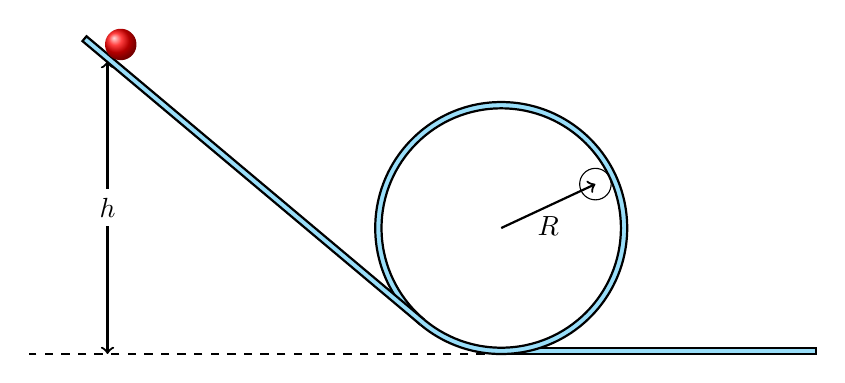
\begin{tikzpicture}[scale=.8,thick]
      \draw[fill=cyan!40] (0,-2) rectangle (5,-1.9);
      \draw[fill=cyan!40] circle (2);
      \draw[fill=white] circle (1.9);
      \begin{scope}[rotate=-40]
        \draw[fill=cyan!40] (0,-2)--(-7,-2)--(-7,-1.9)--(0,-1.9);
        \shade[ball color=red] (-6.5,-1.65) circle (.25);
      \end{scope}
      \draw[dashed] (0,-2)--(-7.5,-2);
      \draw[<->] (-6.25,-2)--(-6.25,2.65) node[midway,fill=white]{$h$};
      \begin{scope}[rotate=25]
        \draw[->] (0,0)--(1.65,0) node[midway,below]{$R$};
        \draw[thin] (1.65,0) circle (.25);
      \end{scope}
    \end{tikzpicture}
    
    \underline{Note:} Diagram not drawn to scale
  }
  \question A uniform ball of radius $r$, with a mass of $M$, and a rotational
  inertia of $I=\dfrac25Mr^2$, rolls without slipping along the loop-the-loop
  track in the figure above. The ball starts at rest at a height of $h$ above
  the bottom of the loop. The radius of the loop is $R$.
  \begin{parts}
    \part\textbf{Determine} the slowest speed that the ball can have without
    leaving the track.
    \vspace{\stretch{.5}}
    
    \part If it is not to leave the track at the top of the loop,
    \textbf{determine} the least value $h$ can have (in terms of radius $R$ of
    the loop)?
    \vspace{\stretch1}
    
    \part What would $h$ have to be if, instead of rolling, the ball slides
    without friction?
    \vspace{\stretch1}
  \end{parts}
  \newpage
  
  \uplevel{
    \centering
    \begin{tikzpicture}[scale=.65]
      \fill[gray!70] circle(1);
      \draw[vectors] (-1,4.5)--(-1,0) arc(180:360:1)--(1,2) node[above]{$F_A$};
      \draw[thick] (-1,0) arc(180:0:1);
      \fill[gray] (-5,4.5) rectangle(4,4.9);
    \end{tikzpicture}
  }
  \question A disk of mass $M =\SI{2.0}{\kilo\gram}$ and radius
  $R=\SI{.10}\metre$ is supported by a rope of negligible mass, as shown
  above. The rope is attached to the ceiling at one end and passes under the
  disk. The other end of the rope is pulled upward with a force $F_A$. The
  rotational inertia of the disk around its center is $MR^2/2$.
  \begin{parts}
    \part\textbf{Calculate} the magnitude of the force $F_A$ necessary to hold
    the disk at rest.
    \vspace{\stretch1}
    
    \uplevel{
      At time $t=0$, the force $F_A$ is increased to 12 N, causing the disk to
      accelerate upward. The rope does not slip on the disk as the disk rotates.
    }

    \part\textbf{Calculate} the linear acceleration of the disk.
    \vspace{\stretch1}
    
    \part\textbf{Calculate} the angular speed of the disk at
    $t=\SI{3.0}\second$.
    \vspace{\stretch1}
    
    \part\textbf{Calculate} the increase in total mechanical energy of the disk
    from $t=0$ to $t=\SI{3.0}\second$.
    \vspace{\stretch1}
    \newpage
    
    \part The disk is replaced by a hoop of the same mass and radius.
    \textbf{Indicate} whether the linear acceleration of the hoop is greater
    than, less than, or the same as the linear acceleration of the disk.

    \vspace{.1in}
    \underline{\hspace{.3in}} Greater than\hspace{.2in}
    \underline{\hspace{.3in}} Less than\hspace{.2in}
    \underline{\hspace{.3in}} The same as

    \vspace{.1in}\textbf{Justify} your answer.
    \vspace{\stretch1}
  \end{parts}
  \newpage
  
  % TAKEN FROM 2005 AP PHYSICS MECHANICS EXAM QUESTION MECH.3 WITHOUT
  % MODIFICATIONS
  \uplevel{
    \centering
    \begin{tikzpicture}[scale=.82,very thick]
      \draw rectangle (4.5,5) node[midway,below=60]{Before Collision};
      \draw[thick,dashed] (2.25,.2)--(2.25,4.8);
      \fill (2.25,1) circle (.15) node[below right]{$M_2$};
      \fill (2.25,4) circle (.07) node[right]{$P$};
      \begin{scope}[rotate around={-30:(2.25,4)}]
        \draw (2.15,4.1) rectangle (2.35,.9) node[midway,below right=-2]{$M_1$};
        \draw[thick,|<->|] (1.8,4.1)--(1.8,.9) node[midway,above left=-3]{$d$};
        \draw[axes] (2.15,.8) arc (270:285:4) node[midway,below left]{$\omega$};
      \end{scope}
    \end{tikzpicture}
    \hspace{.35in}
    \begin{tikzpicture}[scale=.82,very thick]
      \draw rectangle (4.5,5) node[midway,below=60]{After Collision};
      \draw[thick,dashed] (2.25,.2)--(2.25,4.8);
      \fill (2.7,1) circle (.15) node[below=2]{$M_2$};
      \fill (2.25,4) circle (.07) node[right]{$P$};
      \draw (2.15,4.1) rectangle (2.35,.9) node[midway,right]{$M_1$};
      \draw[thick,|<->|] (1.8,4.1)--(1.8,.9) node[midway,left]{$d$};
      \draw[axes] (3,1)--+(1,0);
    \end{tikzpicture}
    
    TOP VIEWS
  }
  \question A system consists of a ball of mass $M_2$ and a uniform rod of mass
  $M_1$ and length $d$. The rod is attached to a horizontal frictionless table
  by a pivot at point $P$ and initially rotates at an angular speed $\omega$ ,
  as shown above left. The rotational inertia of the rod about point $P$ is
  $\frac13M_1d^2$. The rod strikes the ball, which is initially at rest. As a
  result of this collision, the rod is stopped and the ball moves in the
  direction shown above right. Express all answers in terms of $M_1$, $M_2$,
  $\omega$, $d$, and fundamental constants.
  \begin{parts}
    \part\textbf{Derive} an expression for the angular momentum of the rod
    about point $P$ before the collision.
    \vspace{\stretch1}
    
    \part\textbf{Derive} an expression for the speed $v$ of the ball after the
    collision.
    \vspace{\stretch1}
    
    \part Assuming that this collision is elastic, \textbf{calculate} the
    numerical value of the ratio $M_1/M_2$.
    \vspace{\stretch1}
    \newpage
    
    \uplevel{
      \centering
      \begin{tikzpicture}[scale=.82,very thick]
      \draw rectangle (4.5,5) node[midway,below=60]{Before Collision};
      \draw[thick,dashed] (2.25,.2)--(2.25,4.8);
      \fill (2.25,2.5) circle (.15) node[below right]{$M_1$};
      \fill (2.25,4) circle (.07) node[above right]{$P$};
      \draw[thick,|<->|] (2.7,4)--(2.7,2.5) node[midway,right=-2]{$x$};
      \begin{scope}[rotate around={-30:(2.25,4)}]
        \draw (2.15,4.1) rectangle (2.35,.9);
        \draw[thick,|<->|] (1.8,4.1)--(1.8,.9) node[midway,above left=-3]{$d$};
        \draw[axes](2.15,.8)arc(270:285:4) node[midway,below left=-3]{$\omega$};
      \end{scope}
    \end{tikzpicture}
    }
    \part A new ball with the same mass $M_1$ as the rod is now placed a
    distance $x$ from the pivot, as shown above. Again assuming the collision
    is elastic, \textbf{determine} the value of $x$ that the rod stop moving
    after hitting the ball?
  \end{parts}
  \newpage
  
  % TAKEN FROM 2023 AP PHYSICS C MECHANICS EXAM SET 1 QUESTION 3 WITHOUT
  % MODIFICATIONS
  \uplevel{
    \centering
    \pic{.7}{disks}\\
    \underline{Note:} Figure not drawn to scale.
  }
  
  \question A solid uniform disk is supported by a vertical stand. The disk is
  able to rotate with negligible friction about an axle that passes through the
  center of the disk. The mass and radius of the disk are given by $M_\text{d}$
  and $R$, respectively. The rotational inertia of the disk is
  $I_\text{d}=\dfrac12 M_\text{d}R^2$. A string of negligible mass is draped over
  the disk and attached to the top of the disk at point P. One end of the
  string is connected to an unstretched ideal spring of spring constant $k$,
  which is fixed to the ground as shown in Figure 1.
  
  \vspace{.2in}A block of mass $m_\text{B}$ is then attached to the string on
  the right side of the disk. The block is slowly lowered until the
  spring-disk-block system reaches equilibrium, as shown in Figure 2. In this
  equilibrium position, the disk has rotated clockwise through a small angle
  $\theta$.

  \vspace{.2in}Give all algebraic answers in terms of $M_\text{d}$, $R$, $k$ ,
  $\theta$, and physical constants, as appropriate.

  \begin{parts}
    \part\textbf{Derive} an expression for the mass $m_\text{B}$ of the block.
    \vspace{\stretch1}
    \newpage
    
    \part At time $t=0$, the string on the right side of the disk is cut and
    the block falls to the ground. On the circle below, which represents the
    disk, \textbf{draw} and \textbf{label} the forces (not components) that act
    on the disk immediately after the string is cut and the block is falling to
    the ground. Each force should be represented by an arrow that starts on and
    is directed away from the point of application.
    \begin{center}
      \vspace{.2in}
      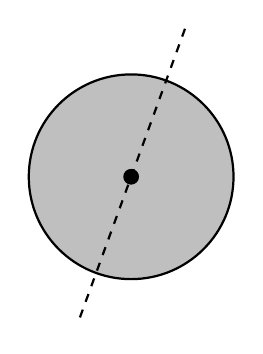
\begin{tikzpicture}
        \draw[thick,fill=lightgray] circle (1.3);
        \fill circle (.1);
        \draw[rotate=-20,dashed,thick] (0,2)--(0,-2);
      \end{tikzpicture}
      \vspace{.2in}
    \end{center}

    \part\textbf{Derive} an expression for the angular acceleration $\alpha$ of
    the disk immediately after the string is cut.
    \vspace{\stretch1}

    \part At $t=t_1$, the disk has rotated and point P is again directly above
    the axle. \textbf{Sketch} a graph of the magnitude of the angular velocity
    $\omega$ of the disk as a function of time $t$ from $t=0$ to $t=t_1$.
    \begin{center}
      \begin{tikzpicture}[thick]
        \draw[->] (0,0)--(8,0) node[right]{$t$};
        \draw[->] (0,0)--(0,6) node[above]{$\omega$};
        \draw[dashed] (5.5,0)--(5.5,5.5) node[pos=0,below]{$t_1$};
      \end{tikzpicture}
    \end{center}
    \newpage
    
    \uplevel{
      \centering
      \pic{.4}{disk2}\\
      \underline{Note:} Figure not drawn to scale.
    }
    \part The disk is adjusted on the support so that the axle does
    \underline{not} pass through the center of mass of the disk. The block is
    again hung on the right side of the disk and the spring-disk-block system
    comes to equilibrium, as shown in Figure 3. The axle does not exert a
    torque on the disk. For each force on the disk, \textbf{indicate} whether
    the magnitude of the torque about the axle caused by that force increases,
    decreases, or stays the same relative to part \textbf{B}. 
  \end{parts}
\end{questions}
\end{document}
